\chapter{Unit testing}

\begin{summary}
De software die we ontwikkelen moet kwaliteitsvol zijn. Maar hoe kunnen we er nu voor zorgen dat we het aantal bugs in onze code zo laag mogelijk houden? E\'en van de strategie\"en om de kwaliteit van software te waarborgen is testen. Testen is een heel belangrijk aspect van softwareontwikkeling waar je ongetwijfeld nog heel veel over gaat leren. 

Als ontwikkelaar zorg je er altijd voor dat wanneer je de gevraagde functionalteit implementeert, je ook de nodige unit testen schrijft om de kwaliteit van je code te garanderen. Wanneer je unit testen schrijft, ga je alle methoden van je klasse testen. Een methode van een klasse is dus de ``unit'' die we gaan testen.
We gaan automatische testen schrijven. Dit betekent dat iedere keer dat de code wordt aangepast of uitgebreid de testen eenvoudig opnieuw kunnen worden uitgevoerd. Op die manier gaan de fouten die ontstaan tijdens de verdere ontwikkeling van de software snel ontdekt worden. Bedenk ook dat een fout, onduidelijkheid of bug die vroeg in het ontwikkelproces wordt aangepakt, maar een kleine impact heeft (ook financieel) ten opzicht van problemen die later pas opduiken.
\end{summary}

\section{JUnit}

In Java gaan we gebruikmaken van het framework JUnit5 om onze unit testen te schrijven.
JUnit5 is opgedeeld in 3 sub-projecten:  Jupiter, Vintage en Platform. JUnit Jupiter is het  sub-project dat wij gebruiken om onze testen te schrijven en voorziet de engine om deze testen uit te voeren.


https://education.launchcode.org/java-web-development/chapters/unit-testing/exercises.html

https://www.didattica.agentgroup.unimo.it/wiki/images/7/7b/Es01-JUnit.pdf

\section{Unit test voor een constructor}

We starten direct met een voorbeeld. In het vorige hoofdstuk hadden we de klasse Documentary aangemaakt. De klasse Documentary is een subklasse van Movie. Bij het aanmaken van een Documentary-object moet wel steeds als genre Genre.DOCUMENTARY ingevuld zijn. 

\begin{lstlisting}
package be.pxl.ja.opdracht1;

public class Documentary extends Movie {

	private String topic;

	public Documentary(String title, Rating rating) {
		super(title, rating);
		addGenre(Genre.DOCUMENTARY);
	}

	public String getTopic() {
		return topic;
	}

	public void setTopic(String topic) {
		this.topic = topic;
	}
}
\end{lstlisting}

We gaan dus de constructor van de klasse Documentary testen.

Onze testklassen gaan we niet mengen met onze eigenlijke programma. Ons hoofdprogramma en de klassen zitten meestal in een source-folder (src). Onze unit testen plaatsen we in een overeenkomstig package in de test-folder. Wanneer je een folder met de naam ``test'' hebt aangemaakt, markeer deze dan ook als test-folder.


\begin{lstlisting}
package be.pxl.ja.opdracht1;

import org.junit.jupiter.api.Test;

import static org.junit.jupiter.api.Assertions.assertEquals;

public class DocumentaryTest {

	private static final String TITLE = "Planet Earth";

	@Test
	public void documentaryConstructor() {
		// ACT
		Documentary documentary = new Documentary(TITLE, Rating.TEENS);

		// ASSERT
		assertEquals(TITLE, documentary.getTitle());
		assertEquals(Rating.TEENS, documentary.getRating());
		assertEquals(Genre.DOCUMENTARY, documentary.getGenre());
	}
}
\end{lstlisting}

\global\csname @topnum\endcsname 0

We hoeven enkel een @Test annotatie toe te voegen opdat een test herkend wordt en uitgevoerd kan worden. De eerste keer dat je de annotatie @Test toevoegt in het project zal deze nog niet gekend zijn. IntelliJ zal zelf voorstellen om JUnit te downloaden en toe te voegen aan het classpath. Zorg er wel voor dat je de juiste versie gebruikt. 


Wanneer je nu de unit test DocumentaryTest uitvoert kunnen er 3 mogelijke scenario's plaatsvinden. Ofwel slaagt de test, ofwel faalt \'e\'en van de beweringen (asserts) ofwel loopt er iets onverwachts fout. In het eerste geval krijgt je test een groene kleurcode, in het tweede scenario een oranje en in het laatste scenario een rode.

\begin{figure}[H]
  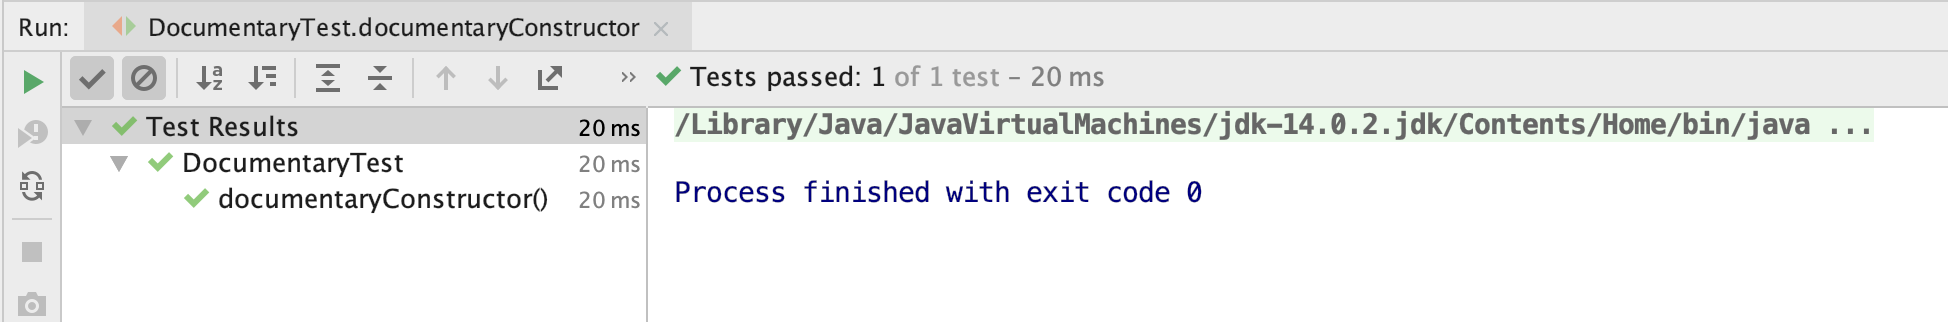
\includegraphics[width=\linewidth]{images/chapter-junit/junit_test_passed.png}
  \caption{Geslaagde JUnit5 test}
  \label{fig:test_passed}
\end{figure}

\begin{figure}[H]
  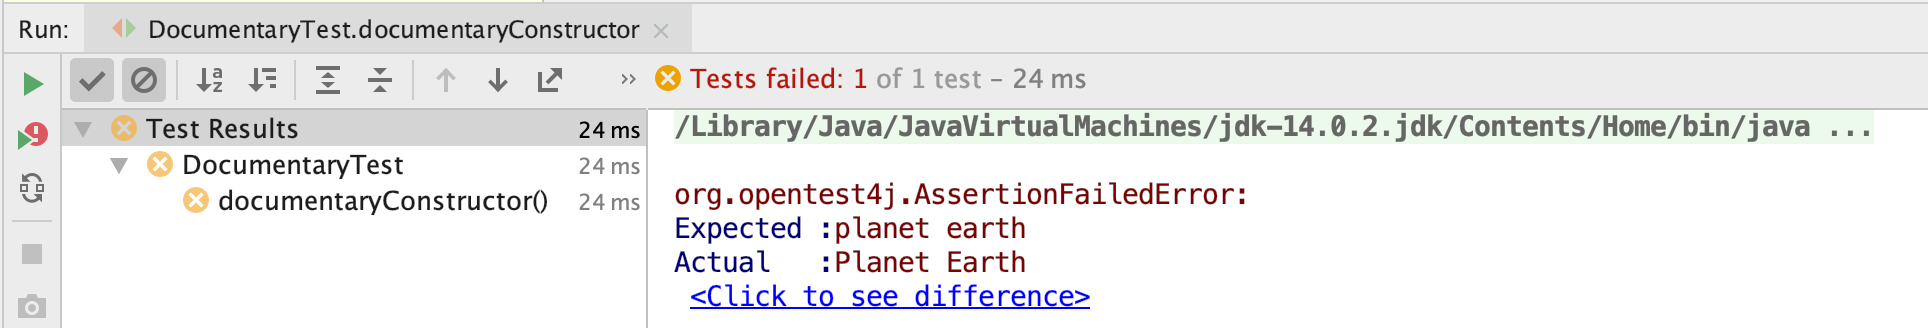
\includegraphics[width=\linewidth]{images/chapter-junit/junit_test_failed.png}
  \caption{Gefaalde JUnit5 test}
  \label{fig:test_failed}
\end{figure}



De methode van de Nederlandse weeramateurs is simpel. Het weercijfer tussen 0 en 10 wordt bepaald uit het weer overdag, tussen 7 en 19 uur. Een droge dag met nauwelijks bewolking of mist en weinig wind krijgt een 10. Afhankelijk van de hoeveelheid wolken vermindert dit met 1 tot 3 punten. Is het mistig dan kost dat, afhankelijk van de duur 1 of 2 punten. Voor de regen telt het aantal uurvakken met neerslag, dus ook alleen de duur. Zijn er tussen 7 en 19 uur twee uurvakken met regen dan kost dat 1 punt. Maar regent het in 11 of 12 uurvakken dan kost dat 4 punten.

Een zwakke wind kost geen punten, maar een matige wind van windkracht 3 gedurende minstens 3 uur kost 1 punt. De temperatuur speelt geen rol, zodat het weercijfer objectief is en ook koude, mooie dagen gunstig scoren. Langdurige regen overdag en veel wind leveren altijd een lage score.

\section{Unit test voor een setter}

Onze test zal steeds opgebouwd worden volgens het 3A patroon: Arrange, Act en Assert.
In iedere test herken je steeds deze 3 bouwstenen. 

Het ``arrange''-gedeelte is waar het object dat getest moet worden en alle andere objecten - die nodig zijn om de test goed uit te voeren - worden aangemaakt. 
Het ``act''-gedeelte is waar we de methode die we willen testen aanroepen. Als de methode een returnwaarde heeft ken je dit toe aan een variabele.

Het ``assert''-gedeelte geeft je de mogelijkheid om beweringen over het resultaat te verifi\"eren.

Hier is nog eens de klasse Movie.

\begin{lstlisting}
import java.time.LocalDate;

public class Movie extends Content implements Playable {
	private String director;
	private LocalDate releaseDate;
	private int duration;

	public Movie(String title, Rating rating) {
		super(title, rating);
	}

	public String getDirector() {
		return director;
	}

	public void setDirector(String director) {
		this.director = director;
	}

	public LocalDate getReleaseDate() {
		return releaseDate;
	}

	public void setReleaseDate(LocalDate releaseDate) {
		this.releaseDate = releaseDate;
	}

	public int getDuration() {
		return duration;
	}

	@Override
	public void play() {
		System.out.println("Playing " + this);
	}

	@Override
	public void pause() {
		System.out.println("Pausing " + this);
	}

	public boolean isLongPlayingTime() {
		return duration > LONG_PLAYING_TIME;
	}

	public String getPlayingTime() {
		// TODO: implement this method correctly		
		return "2 u 30 min";
	}

	@Override
	public String toString() {
		StringBuilder builder = new StringBuilder(super.toString());
		if (releaseDate != null) {
			builder.append(" (").append(releaseDate.getYear()).append(")");
		}
		return builder.toString();
	}
}
\end{lstlisting}

\global\csname @topnum\endcsname 0

Bekijk de methode void setDuration(int duration) eens. We willen nooit een negatief getal als waarde voor de eigenschap duration. Daarom zullen we de absolute waarde nemen van de parameter duration. Om deze setter te testen gaan we 2 testen voorzien. Een eerste test waar we een positieve waarde meegeven als argument en een tweede test waarbij we een negatieve waarde meegeven.

\begin{lstlisting}
import org.junit.jupiter.api.Test;

import static org.junit.jupiter.api.Assertions.assertEquals;

public class MovieSetDurationTest {

	@Test
	public void negativeDurationBecomesPositive() {
		// ARRANGE
		Movie movie = new Movie("Titanic", Rating.OLDER_KIDS);

		// ACT
		movie.setDuration(-125);

		// ASSERT
		assertEquals(125, movie.getDuration());
	}

	@Test
	public void positiveDurationStaysUnchanged() {
		// ARRANGE
		Movie movie = new Movie("Titanic", Rating.OLDER_KIDS);

		// ACT
		movie.setDuration(125);

		// ASSERT
		assertEquals(125, movie.getDuration());
	}
}
\end{lstlisting}

\clearpage

\section{Unit test voor een getter}

In de klasse Movie vind je ook de methode isLongPlayingTime() terug. Deze methode heeft een boolean als resultaat-type en geeft true indien de film langer dan 2 u 15 min duurt.

Hier is alvast 1 mogelijke unit test.

\begin{lstlisting}
import static org.junit.jupiter.api.Assertions.assertFalse;

public class MovieIsLongPlayingTimeTest {
	
	@Test
	public void movieWithDurationShorterThanLongPlayingTimeReturnsFalse() {
		
		Movie movie = new Movie("Titanic", Rating.TEENS);
		
		movie.setDuration(Movie.LONG_PLAYING_TIME - 1);
		
		assertFalse(movie.isLongPlayingTime());
	}
}
\end{lstlisting}

Bij de overige testen zullen in het Arrange gedeelte opnieuw een Movie-object moeten aanmaken. Omdat dit voor iedere test herzelfde is, hoeven we deze code niet te dupliceren. 
Met de annotatie @BeforeEach kunnen we een methode aanduiden die wordt uitgevoerd voor elke test.

Daarnaast merk je ook dat de klasse org.junit.jupiter.api.Assertions bijkomende static methoden heeft om de resultaten van de test te verifi\"eren. \textbf{assertFalse} en \textbf{assertTrue} zullen  slagen als de getestte waarde repectievelijk false of true is.

\begin{lstlisting}
import org.junit.jupiter.api.BeforeEach;
import org.junit.jupiter.api.Test;

import static org.junit.jupiter.api.Assertions.assertFalse;
import static org.junit.jupiter.api.Assertions.assertTrue;

public class MovieIsLongPlayingTimeTest {

	private Movie movie;

	@BeforeEach
	public void init() {
		movie = new Movie("Titanic", Rating.TEENS);
	}

	@Test
	public void movieWithDurationShorterThanLongPlayingTimeReturnsFalse() {

		movie.setDuration(Movie.LONG_PLAYING_TIME - 1);

		assertFalse(movie.isLongPlayingTime());
	}

	@Test
	public void movieWithDurationExactlyLongPlayingTimeReturnsFalse() {

		movie.setDuration(Movie.LONG_PLAYING_TIME);

		assertFalse(movie.isLongPlayingTime());
	}

	@Test
	public void movieWithDurationLongerThanLongPlayingTimeReturnsTrue() {

		movie.setDuration(Movie.LONG_PLAYING_TIME + 1);

		assertTrue(movie.isLongPlayingTime());
	}
}
\end{lstlisting}

We maken ook in de testen handig gebruik van de constante LONG\_PLAYING\_TIME. Door onze testen op deze manier te schrijven hoeven we de testen niet aan te passen als de waarde van LONG\_PLAYING\_TIME wordt aangepast. 

Hier is een overzicht van enkele handige static methoden uit de klasse org.junit.jupiter.api.Assertions. 

\begin{table}[h!]
\centering
\begin{tabularx}{\textwidth}{| l | X |}
 \hline
 Methode & Betekenis\\ 
 \hline\hline
assertEquals() & Evalueert de gelijkheid van 2 waarden. De test slaagt als beide
waarden gelijk (equal) zijn.\\
\hline
assertFalse() & Evaluatie van een booleaanse uitdrukking. De test slaagt indien
de uitdrukking false is.\\
\hline
assertTrue() & Evaluatie van een booleaanse uitdrukking. De test slaagt indien
de uitdrukking true is.\\
\hline
assertNotNull( ) & Vergelijkt een object referentie met null. De test slaagt indien de
object referentie niet null is.\\
\hline
assertSame( ) & Vergelijkt het geheugenadres van twee object referenties
(gebruik maken van == operator). De test slaagt indien beide
object referenties naar hetzelfde object verwijzen.\\
\hline
fail() & Zorgt ervoor dat de test zal falen.\\
 \hline
\end{tabularx}
\caption{Static methoden uit de klasse org.junit.jupiter.api.Assertions}
\label{table:assertions}
\end{table}

\begin{oefening}
Schrijf 2 unit testen voor de toString() methode van de klasse Movie. We verwachten dat deze methode de titel en het jaartal van de film teruggeeft (bijv. Titanic (1997)). Indien er geen releasedatum gekend is, wordt het jaartal achterwege gelaten.
\end{oefening}

\begin{oefening}
Schrijf unit testen voor de methode addGenre in de klasse Content. Let er ook op dat een  genre enkel wordt toegevoegd indien het niet eerder al werd toegevoegd. 
\end{oefening}

\begin{oefening}
Je ziet dat in bovenstaande klasse Movie de methode getPlayingTime() nog niet correct ge\"implementeerd is. Hier zijn alvast de unit testen. 

\begin{lstlisting}
import org.junit.jupiter.api.BeforeEach;
import org.junit.jupiter.api.Test;

import static org.junit.jupiter.api.Assertions.assertEquals;

public class MovieGetPlayingTimeTest {

	private Movie movie;

	@BeforeEach
	public void init() {
		movie = new Movie("Titanic", Rating.OLDER_KIDS);
	}

	@Test
	public void returnsQuestionmarkWhenDurationZero() {

		movie.setDuration(0);

		assertEquals("?", movie.getPlayingTime());
	}

	@Test
	public void returnsMinutesWhenDurationLessThan60() {

		movie.setDuration(59);

		assertEquals("59 min", movie.getPlayingTime());
	}

	@Test
	public void returnsHoursWhenDurationMultipleOf60() {

		movie.setDuration(120);

		assertEquals("2 h", movie.getPlayingTime());
	}

	@Test
	public void returnsHoursAndMinutesWhenDurationNotMultipleOf60() {

		movie.setDuration(135);

		assertEquals("2 h 15 min", movie.getPlayingTime());
	}
}
\end{lstlisting}

Bestudeer deze unit testen en implementeer vervolgens de methode. Test je implementatie uit! Wanneer alle testen slagen, bekijk dan je je code nog eens kritisch. Kan je nog verbeteringen aanbrengen in de code?
\end{oefening}

Je ziet dat je geen schrik moet hebben om achteraf je code te verbeteren. Omdat je beschikt over unit testen kan je rustig aan je code gaan sleutelen. Het proces om code te verbeteren en hierdoor de leesbaarheid en onderhoudbaarheid van de code te verhogen noemen we \textbf{refactoren}. 

\begin{remark}
  Meer weten over unit testing, kijk op pluralsight: \url{https://app.pluralsight.com/library/courses/junit-5-unit-testing-getting-started}
\end{remark}

\begin{oefening}
We gaan bij de domeinklassen van de streaming service nog enkele klassen en enums toevoegen. Deze klassen gaan we hergebruiken tijdens latere oefeningen. 

Je implementeert volgende enums en klassen in je oplossingen van opgave 1:
\begin{itemize}
\item CreditCardType
\item PaymentInfo
\item StreamingPlan
\item Profile
\item Account
\end{itemize}

\textbf{Enum CreditCardType}

CreditCardType is een eenvoudige enum-klasse met de waarden VISA en MASTERCARD.

\textbf{Klasse PaymentInfo}

Wanneer een gebruiker een account aanmaakt voor onze streaming service moet hij zijn betaalgegevens opgegeven. Deze gegevens houden we bij in een PaymentInfo-object.
Deze klasse bevat de volgende eigenschappen:

\begin{itemize}
\item cardNumber (String)
\item type (CreditCardType)
\item firstName (String)
\item lastName (String)
\item expirationDate (LocalDate)
\item securityCode (int)
\end{itemize}

Je hoeft enkel getters en setters te voorzien. Het valideren van cardNumber, securityCode en expirationDate houden we voor het volgende hoofdstuk wanneer we het hebben over foutafhandeling.

\textbf{Enum StreamingPlan}

Er zijn 3 producten waaruit gebruikers kunnen kiezen. Ieder product heeft een maximum aantal profielen per account en een prijs. 

Gebruikers met product BASIC kunnen maar 1 profiel aanmaken en betalen €7,99.
Gebruikers die kiezen voor STANDAARD kunnen 2 profielen aanmaken en betalen €11,99.
Tenslotte kunnen gebruikers met een PREMIUM account 4 profielen aanmaken. Zij betalen €15,99.

Maak een enum met de naam StreamingPlan met deze producten. Gebruik numberOfProfiles en price als eigenschappen voor deze enum-klasse. 

\textbf{Klasse Profile}

Afhankelijk van de StreamingPlan kunnen er dus profielen toegevoegd worden aan een account. Daarom implementeren we de klasse Profile. Voor iedere Profile-object willen we een naam (name) en een geboortedatum (dateOfBirth) weten. Deze laatste hebben we nodig om te beslissen of Content beschikbaar is of niet. 

Hiervoor voorzie je een methode \textit{boolean allowedToWatch(Content content)} in de klasse Profile. De methode geeft true als de content geschikt is voor het profiel (afhankelijk van de rating van de content en de geboortedatum van het profiel). 
De methode geeft false als de content niet geschikt is voor het profiel.
Zolang de geboortedatum niet is ingevuld is alle content niet geschikt voor het profiel.
Voeg de nodige unit testen toe om deze methode grondig te testen!

\textbf{Klasse Account}

En tenslotte voeg je de klasse Account toe. Een account heeft volgende eigenschappen:
\begin{itemize}
\item email
\item password
\item streamingPlan
\item \'e\'en of meerder profielen
\item paymentInfo
\end{itemize}

In de constructor van een Account wordt er direct 1 profiel aangemaakt met de naam "profile1" en geboortedatum 1/1/2000. Schrijf unit testen voor de constructor.

De methode getFirstProfile() geeft het eerste (en voorlopig ook enige) Profile-object terug als resultaat. 

De functionaliteit om profielen toe te voegen wordt in een volgend hoofdstuk toegevoegd.

\textbf{Optioneel: Sterkte van het paswoord}

Wanneer de gebruiker een account aanmaakt kiest hij een paswoord. We geven hem graag een indicatie of zijn gekozen paswoord voldoende sterk is.
Maak een hulpklasse \textbf{PasswordUtil}  met een static methode \textit{int calculateStrength(String password)}. 

Hier zijn de regels voor de berekening van de sterkte van een paswoord:
\begin{itemize}
\item Een paswoord met minder dan 6 karakters is zwak en geeft altijd een score van 0.
\item Een paswoord met een lengte tussen 6 en 10 geeft een score van 1.
\item Een paswoord met meer dan 10 karaketer geeft een score van 2.
\end{itemize}
Voor paswoorden met een lengte vanaf 6 karakters gelden de volgende bijkomende regels:
\begin{itemize}
\item Indien het paswoord minstens 1 cijfer bevat, wordt de score met 2 verhoogd.
\item Indien het paswoord minstens 1 kleine letter bevat, wordt de score met 2 verhoogd.
\item Indien het paswoord minstens 1 hoofdletter bevat, wordt de score met 2 verhoogd.
\item Indien het paswoord minstens 1 special karakter bevat, wordt de score met 2 verhoogd. Er is reeds een constante aanwezig in de klasse PasswordUtil die de speciale karakters bevat.
\end{itemize}
Implementeer deze regels en schrijf de nodige unit testen.
\end{oefening}

TODO klassendiagram